\documentclass[11pt]{article}
\usepackage{amsmath, textcomp, amssymb, graphicx, parskip, listings}
\usepackage[margin=1.00in]{geometry}

\title{\vspace{-8ex} CS280 Project Proposal \vspace{-8ex}}
\date{}

\begin{document}
\maketitle

\begin{center}
\author{Rohan Chitnis ID\#23464697 ronuchit@berkeley.edu, Alan Yao ID\#23775635 alanyao@berkeley.edu, Alexander Chu ID\#23460953 alex.p.chu@berkeley.edu}
\end{center}

3d graphics on monitors are unrealistic because they assume a center of projection some distance away from the center of the screen. That is, they assume the viewer is at a certain position (usually in front of the middle of the screen) when generating the projection. If the position of the viewer is known, however, the center of projection can be set to match the viewer's point of view. This means looking at the monitor will be much akin to looking through a window. 

We plan to use object recognition to detect the position of the viewer's face using a laptop webcam, using any modern algorithm, calibrating the camera to find focal distance at the same time. In order to achieve online tracking (at 60fps), we will use a faster multi-scale ssd template matching implementation to determine the location of the face. Additionally, we will incorporate rotation and scale invariant matching to find face orientation and distance. To account for the delay between detection frames, we will use a kalman filter to predict and smooth the position of the face when no detection data is available. We will then render a 3d scene using the position of the center of the viewer's face as the center of projection, and adjust the camera up and viewing vectors, along with the location of the camera accordingly.

Shown below are some mock inputs and outputs:

\begin{tabular}[pos]{| l | c | r |}
\hline
Input Scene & Input Position & Output Image
\\ \hline
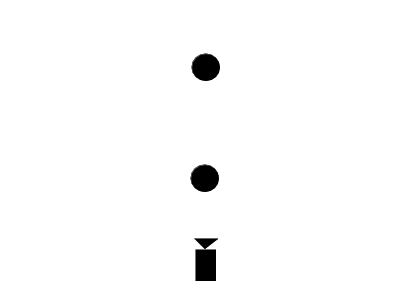
\includegraphics[width=0.33\textwidth]{./img/input_scene1.png}
&
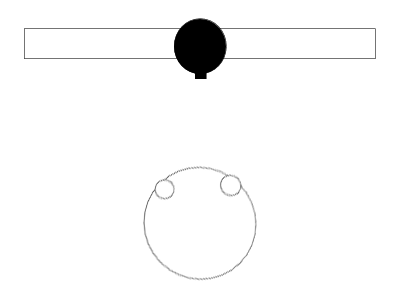
\includegraphics[width=0.33\textwidth]{./img/input_position1.png}
&

\includegraphics[width=0.33\textwidth]{./img/output1.png}
\\ \hline
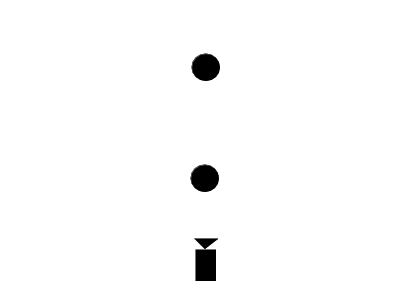
\includegraphics[width=0.33\textwidth]{./img/input_scene2.png}
&
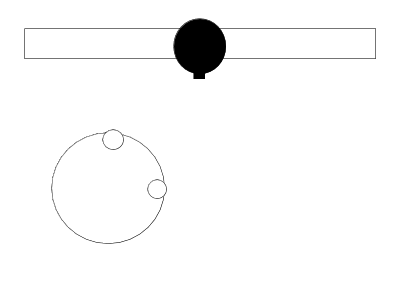
\includegraphics[width=0.33\textwidth]{./img/input_position2.png}
&

\includegraphics[width=0.33\textwidth]{./img/output2.png}
\\ \hline
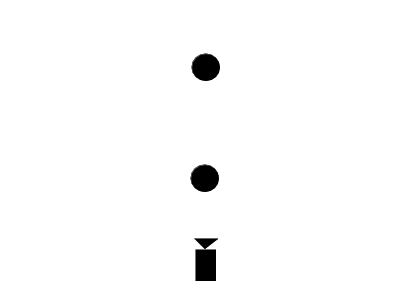
\includegraphics[width=0.33\textwidth]{./img/input_scene3.png}
&
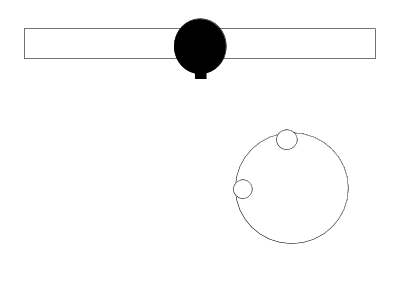
\includegraphics[width=0.33\textwidth]{./img/input_position3.png}
&

\includegraphics[width=0.33\textwidth]{./img/output3.png}
\\ \hline
\end{tabular}
\end{document}
